\begin{figure}[ht]
    \centering
    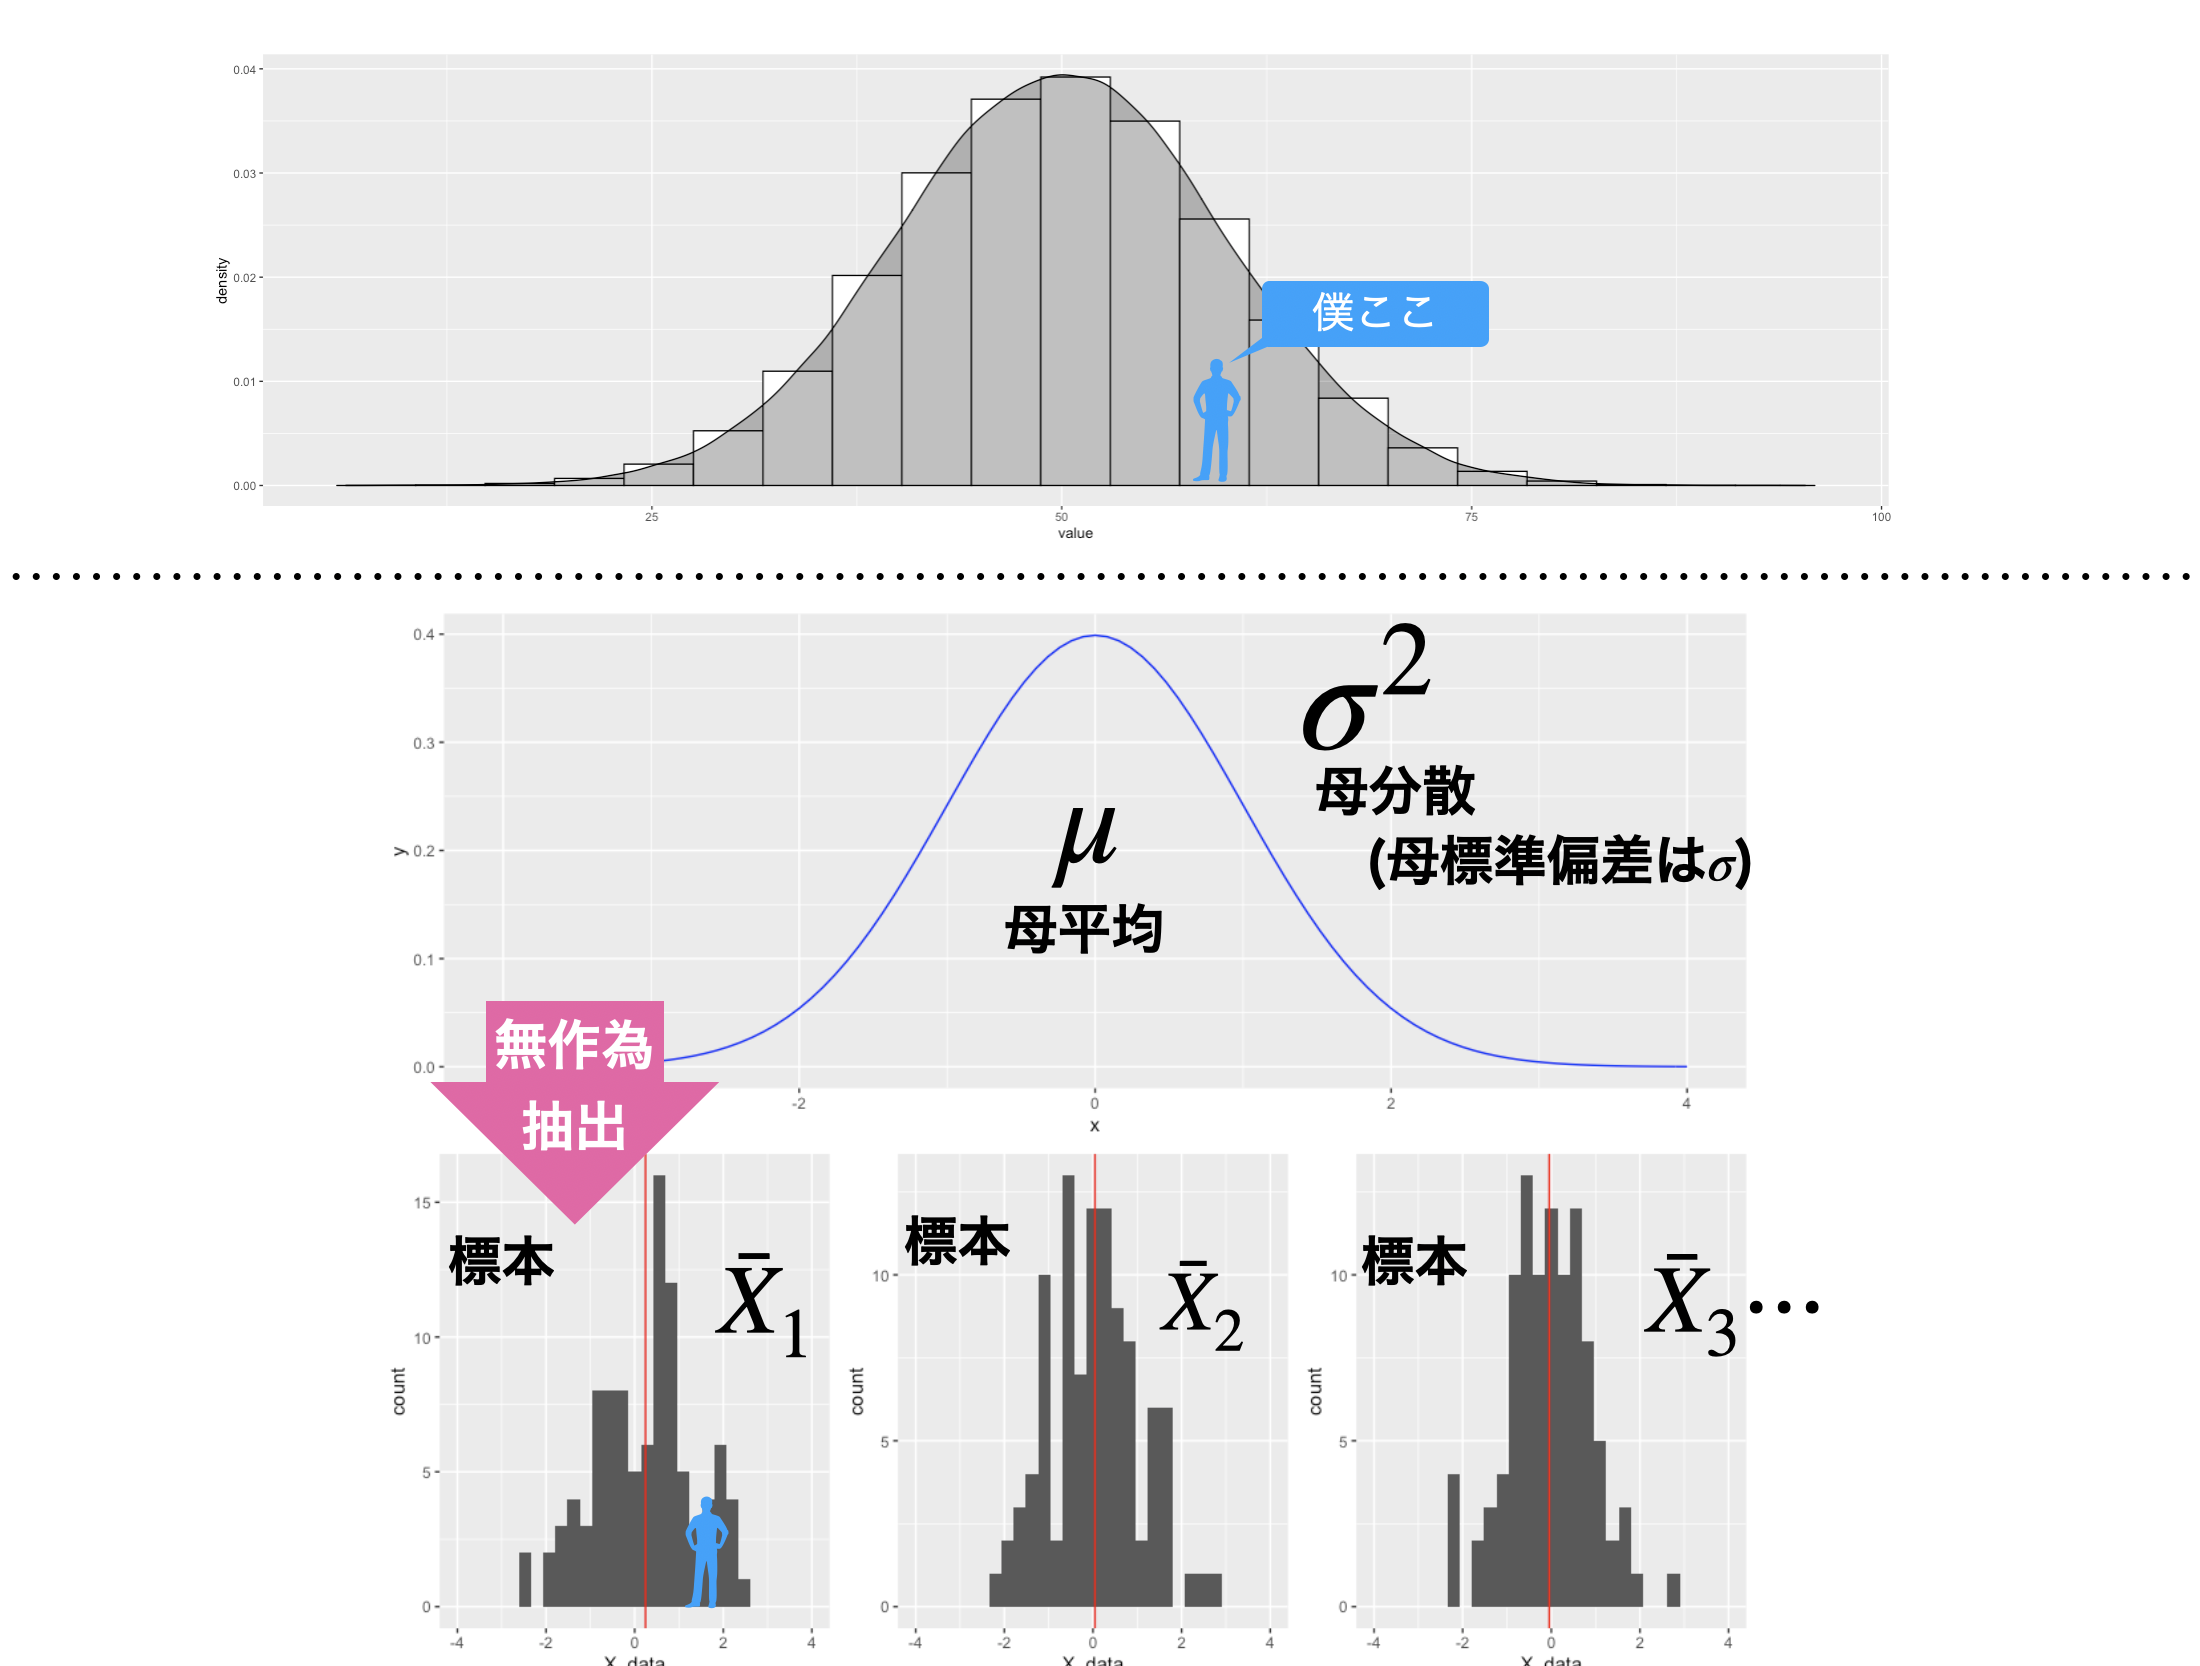
\includegraphics[keepaspectratio,height=0.6\linewidth]{../images/17_estimation_and_test/slide17_1.png}
    \caption{Note that we are considering the framework of inferential statistics. Previously (in Section \ref{UsefulNormal}), we talked about not inferring but positioning an individual score within the population itself and considering its relative position, as shown in the top figure. This time, we are assuming that the population follows a normal distribution and are considering the sample obtained from it, as shown in the bottom figure. Each individual data point is within the sample. Furthermore, we are considering sample statistics, which follow the sample distribution.}
    \label{fig::17_01}
\end{figure}
